DNS queries have historically been unencrypted, leaving users susceptible to eavesdropping; queries can also be intercepted and manipulated~\cite{jones2016detecting}. To address these privacy and security vulnerabilities, encrypted DNS protocols have been developed and deployed, including DNS-over-HTTPS (DoH)~\cite{rfc8484}.

Most contemporary deployments of DoH have occurred in browsers that provide limited options for resolvers~\cite{chromeResolvers,ffChoices}. Although DoH protects against on-path eavesdropping, it does not prevent resolvers themselves from seeing the contents of DNS queries. Thus, some have argued that browser-based DoH deployments shift privacy concerns from eavesdroppers to potential misuse by major DNS providers~\cite{vixie}.

Cloudflare, Cloudflare, Quad9, NextDNS, CleanBrowsing, and OpenDNS are the DoH resolvers that have been deployed
to users of major browsers as of April 14,
2025.  We
define these resolvers as {\em
mainstream}.
Yet, many other DoH resolvers have been deployed that are currently
not in use by major browser deployments~\cite{dnscrypt}---in other words,
there are many non-mainstream DoH resolver deployments.  

Previous studies have measured encrypted DNS performance, but they have mostly focused on mainstream DNS resolvers~\cite{hounsel2020comparing,hounsel2021can,hoang2020k,lu2019end-to-end}.
In this paper, we expand on these previous studies, exploring the performance of all encrypted DNS resolvers—from a variety of global
vantage points, as opposed to simply characterizing the mainstream DoH providers from well-connected vantage points. Our goal is to compare the performance of encrypted DNS resolvers to each other, to understand the extent to which this larger set of DNS resolvers could be used by clients and applications in different regions. 

Importantly, while some large mainstream resolvers (e.g., Google, Cloudflare, Quad9, Hurricane Electric) are anycasted, many smaller and non-mainstream resolvers are not. Thus, our use of geolocation information is not intended as a perfect ground truth of server placement, but rather as a way to group resolvers and provide a more comprehensive set of measurements across vantage points. The focus of this work is not to test geographic placement itself, but to understand performance as experienced by clients.

We make the following contributions: (1) We measure DoH response times a large list of resolvers, including both mainstream DoH resolvers that are included in major browser vendors and a large collection of non-mainstream resolvers. (2) We study how the performance of various DoH resolvers differ based on vantage point. (3) We study the performance of DoH resolvers in home networks. To our knowledge, this paper presents the first study of DoH performance measurements for non-mainstream resolvers, as well as the first comparison of DoH performance across a variety of vantage points, for a large number of resolvers. To perform these experiments, we developed and released an open-source tool for measuring encrypted DNS performance to replicate and extend these results, and to support further research on DoH performance.

We perform measurements across 74 DoH resolvers, grouped by their geographical locations—18 in North America, 13 in Asia, 5 in Australia, and 34 in Europe. 5 resolvers were unable to return a location. These resolvers were scraped from a list of public DoH resolvers provided by the DNSCrypt protocol developers. We employed MaxMind’s GeoLite2 databases to geolocate each DoH resolver. We also took the four highest performing resolvers (Google, Cloudflare, Quad9, Hurricane Electric) located in North America and measured their performance in Europe and Asia to better understand how they compare in farther vantage points. We issued queries for three domains to each resolver: google.com, amazon.com, and wikipedia.com. Our selection of domains is quite realistic, because it is reasonable to expect that most people query sites that are already in cache. 

We define DNS query response time as the
end-to-end time it takes for a client to initiate a query and receive a
response.  To measure query response times with various DoH resolvers, we
performed dig queries to the resolvers. We used the public, open-source Netrics
platform to conduct periodic measurements. Netrics
provides a variety of open-source network measurement tests, and we added our 
test to this suite. 

We performed network latency measurements for each recursive resolver.  Each time
we issued a set of DoH queries to a resolver, we also issued a ICMP ping
message and noted the round-trip time.  This enabled us to explore
whether there was a consistent relationship between high query response times
and network latency.

We collect continuous measurements via two sources—-home network devices and Amazon EC2 instances. The home network measurements were across four units in the same apartment complex in the Chicagoland area, collected between June 22--September 30, 2023. 
We installed our measurement platform on Raspberry Pi devices, which we used to  collect data. 
For the EC2 measurements, we deployed one server
in each of the Ohio, Frankfurt, and Seoul EC2 regions.  We chose to perform
measurements from multiple global vantage points to understand how DoH
performance varies not only by which resolver is used, but also which
geographic region the client is located in.  Each server utilized 8 GB of RAM
and 2 virtual CPU cores (the \texttt{t2.xlarge} instance type), and they each
used Linux/UNIX.

\begin{figure}[!htbp]
\centering
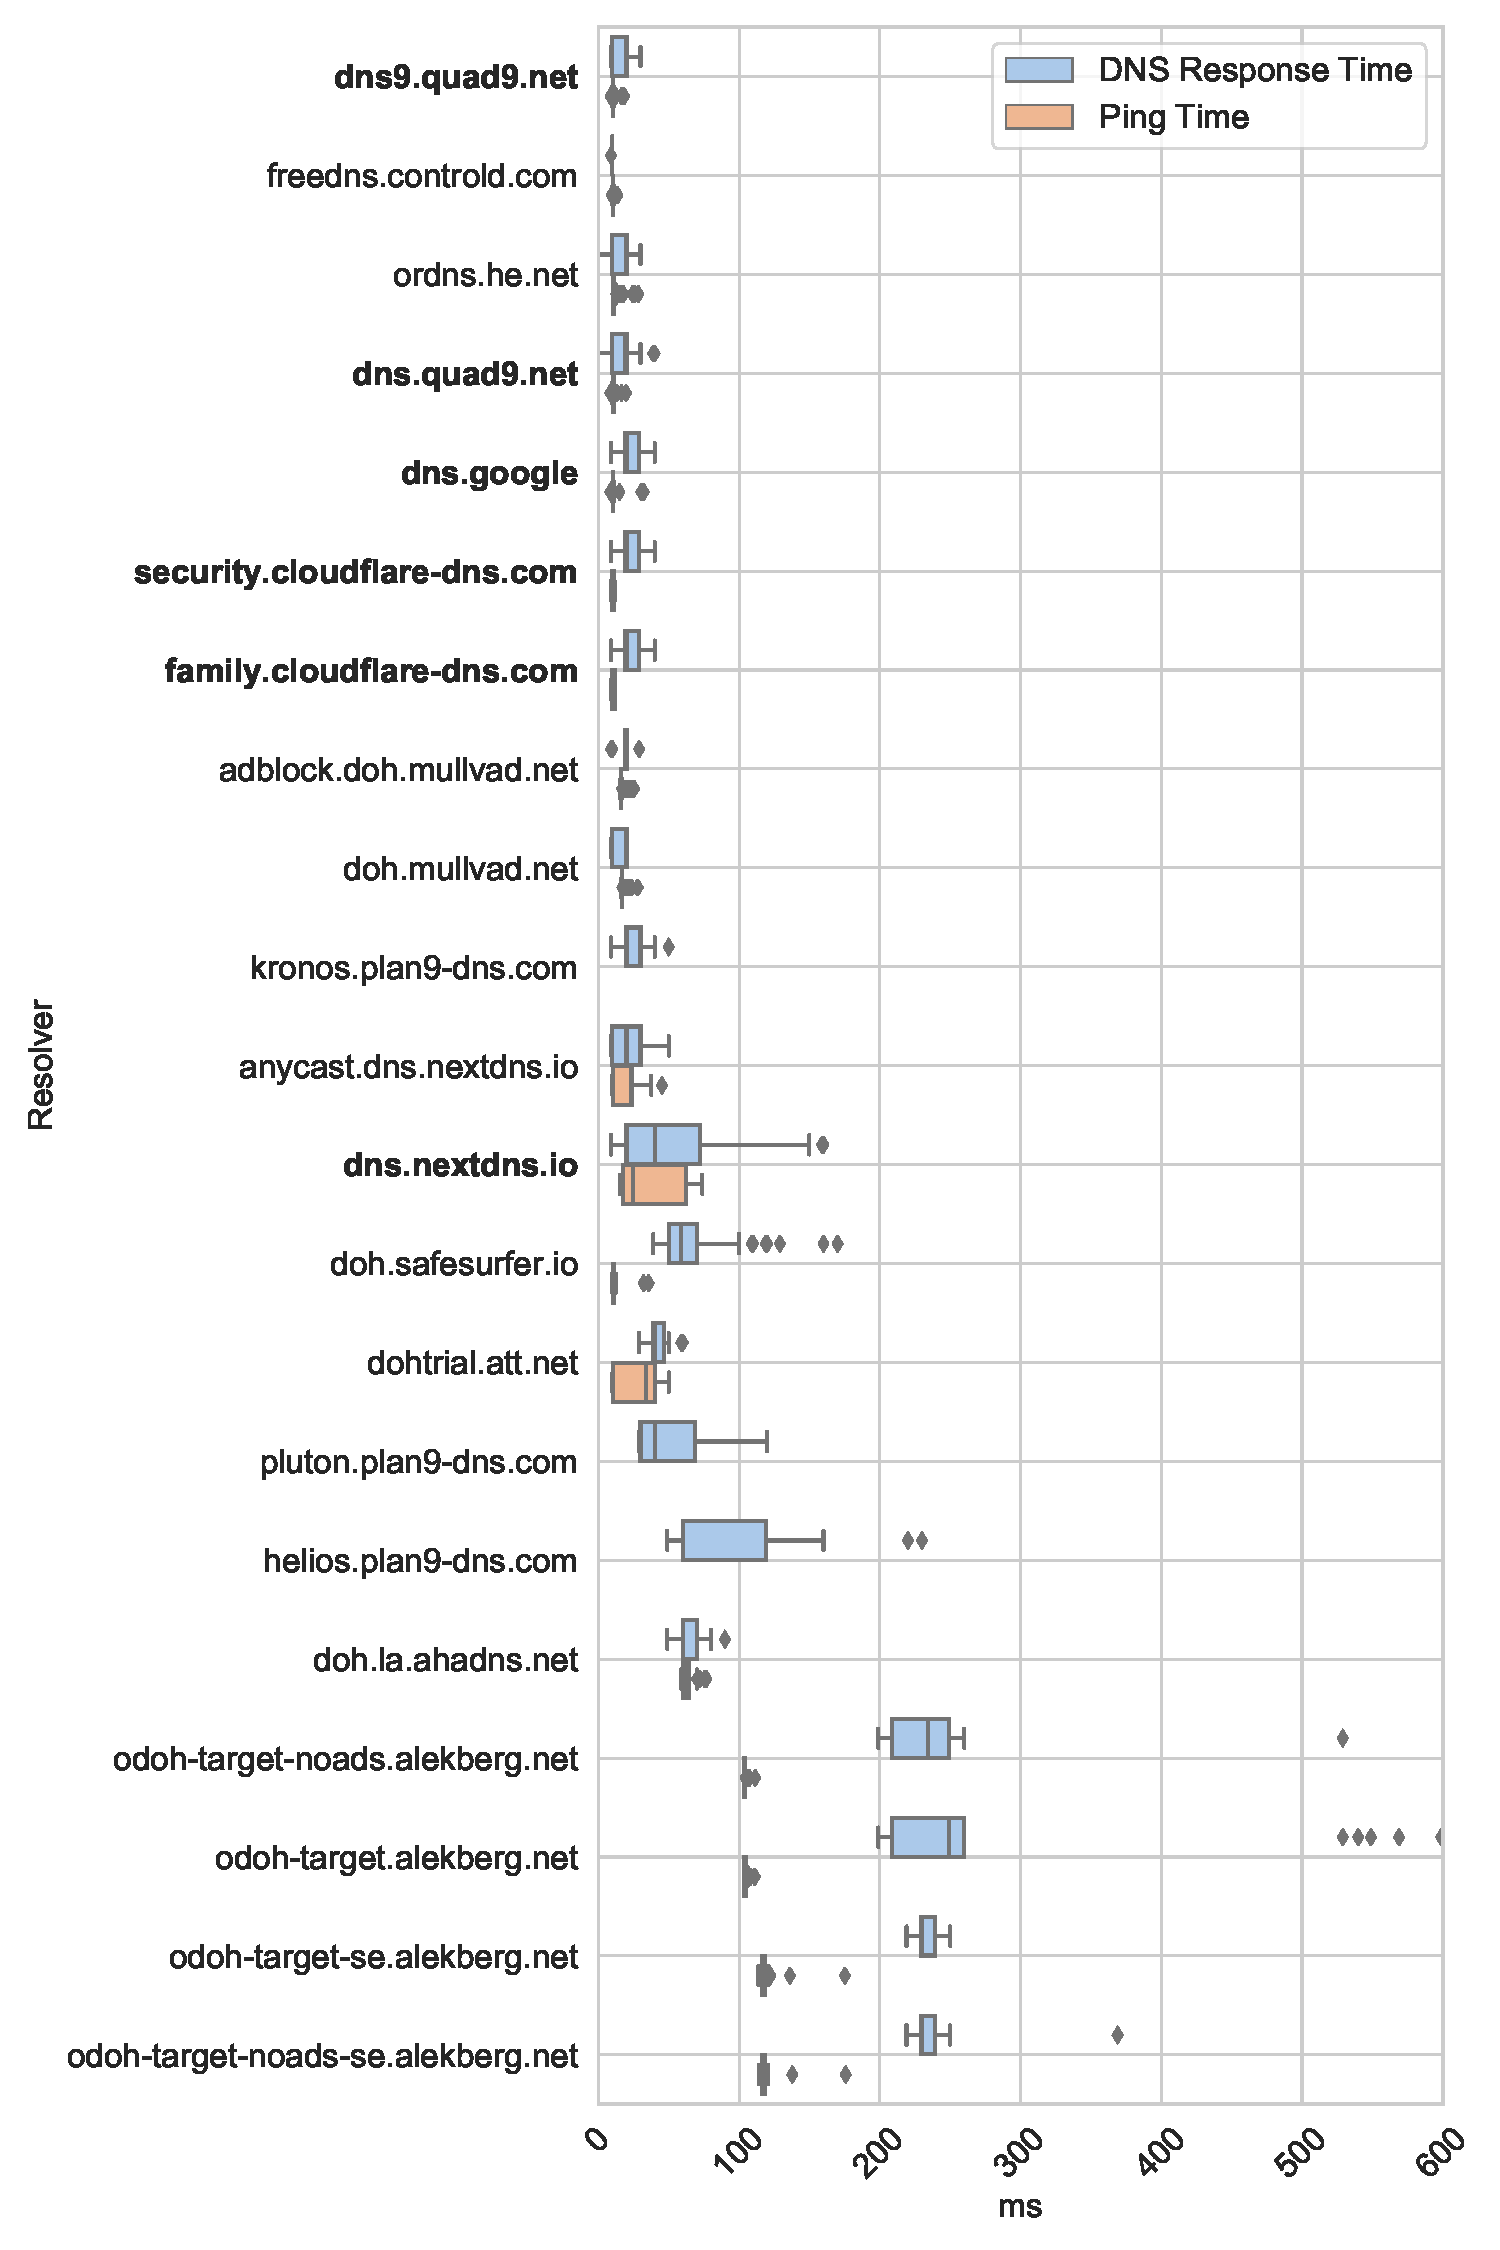
\includegraphics[width=0.6\columnwidth]{figures/ohio_NA.pdf}
\caption{DNS response time and ICMP ping time distributions for
    encrypted DNS resolvers located in North America, measured from EC2 in Ohio. Mainstream resolvers are bolded.}
    \label{fig:dns-us-ohio}
\end{figure}

Figure~\ref{fig:dns-us-ohio} shows the distributions of DNS response times and
ICMP ping times across encrypted DNS resolvers located in North America, as
measured from an EC2 instance in Ohio. The plots show distributions for both DNS response times and ICMP round-trip latency.

As expected, most mainstream resolvers outperformed non-mainstream resolvers from most vantage points. Non-mainstream resolvers also exhibited higher variability of median query response times. In some cases, however, a local non-mainstream resolver can exhibit equivalent performance as compared mainstream resolvers (e.g., ordns.he.net, freedns.controld.com, dns.brahma.world, and dns.alidns.com). These results suggest both good news and room for improvement in the future: On the one hand, viable alternatives to mainstream encrypted DNS resolvers do exist. On the other hand, users need easy ways of finding and selecting these alternatives, whose availability and performance may be more variable over time than mainstream resolvers.

\begin{table}[t!]
\centering
\scriptsize
\begin{tabular}{l|rr}
\toprule
    \textbf{Resolver} & \multicolumn{2}{c}{\textbf{Vantage Point}} \\
                  & \textrm{Seoul (ms)}         & \textrm{Frankfurt (ms)} \\
\midrule
antivirus.bebasid.com                                & 99 & 380                            \\
dns.twnic.tw                          & 59                                          & 290                              \\
dnslow.me                                & 29                                           & 240                              \\
jp.tiar.app                            & 39                                           & 250                             \\
public.dns.iij.jp                              & 39.5                                           & 250                               \\
\bottomrule
\end{tabular}
    \caption{Median DNS response times for non-mainstream resolvers (Asia).}
\label{tab:UnconvAsia}
\end{table}

\begin{table}[t!]
\centering
\scriptsize
\begin{tabular}{l|rr}
\toprule
\textbf{Resolver} & \multicolumn{2}{c}{\textbf{Vantage Point}} \\
                  & \textrm{Frankfurt (ms)}     & \textrm{Seoul (ms)} \\
\midrule
doh.ffmuc.net                               & 70 & 569                         \\
dns0.eu                        & 20 & 399                         \\
open.dns0.eu         & 10 & 324                         \\
kids.dns0.eu                                 & 10 & 309                         \\
dns.njal.la                        & 20 & 289                         \\
\bottomrule
\end{tabular}
    \caption{Median DNS response times for non-mainstream resolvers (Europe).}
\label{tab:UnconvEur}
\end{table}


To better understand the extent to which certain encrypted DNS resolvers
perform, we identified
resolvers that exhibited low DNS response times for clients in one region
but not others. 
Tables~\ref{tab:UnconvAsia} and~\ref{tab:UnconvEur} show 
the five encrypted DNS resolvers for Europe and Asia that exhibit the 
largest differences in median DNS response times when
queried from a remote vantage point (queries of resolvers in Asia from Europe,
and of resolvers of Europe from Asia, respectively). In both cases, 
Table~\ref{tab:UnconvAsia} shows that non-mainstream resolvers located
in Asia perform better from the vantage point in Seoul than the one in
Frankfurt.  Similarly, as expected, Table~\ref{tab:UnconvEur} shows that the
median response times of non-mainstream resolvers in Europe are much lower when
measured from Frankfurt than the response times of those same resolvers
measured from Seoul.

These findings highlight promising advancements and areas for further development. Mainstream DoH deployments by major browser vendors have evidently established a robust encrypted DNS infrastructure, with strong performance, offering improved privacy and security. However, the broader ecosystem of non-mainstream encrypted DNS resolvers presents a more nuanced picture. 
It is also clear that there is an opportunity
to invest in deploying and maintaining reliable, performant, global encrypted
DNS infrastructure operated by a greater diversity of organizations.
